\documentclass[aps, reprint,amsmath,amssymb]{revtex4-1} %APS Journal
\usepackage[T1]{fontenc}
\usepackage[utf8]{inputenc}
\usepackage{lmodern}
\usepackage{microtype}
\usepackage{graphicx}
\usepackage{siunitx}
\usepackage{bm}

\renewcommand{\vec}[1]{\mathbf{#1}}
\newcommand{\mat}[1]{\mathbf{#1}}
\newcommand{\uv}[1]{\vec{\hat{#1}}}
\newcommand{\x}{\vec{\hat{x}}}
\newcommand{\y}{\vec{\hat{y}}}
\newcommand{\z}{\vec{\hat{z}}}
\renewcommand{\d}{\partial}
\renewcommand{\L}{\mathcal{L}}
\renewcommand{\inf}{\infty}

\begin{document}
%----------------------------------------------------------------------
% title
%----------------------------------------------------------------------
\title{PHY64 Experiment 2: The Millikan Oil-drop Experiment}
\author{Matthew S. E. Peterson}
\author{Jackson Burzynski}
\affiliation{Department of Physics and Astronomy, Tufts University}
%\date{\today} 
\maketitle

%----------------------------------------------------------------------
% Body
%----------------------------------------------------------------------
\section{Introduction}

In 1910, American physicist Robert Millikan performed the first experiment to determine the elusive value of the electron charge. Using a microscope, Millikan observed small oil droplets as they fell through two horizontal metal electrodes. He first calculated their terminal velocity with no voltage applied to determine the radius of the droplets. Then, using the known density of the oil, Millikan was able to calculate their mass and therefore the gravitational force on each droplet. Next Millikan applied a voltage between the plates to induce an electric field. By observing the motion of a the droplets in several charge states, Millikan showed that the charges were all small integer multiples of a certain base value. Millikan calculated this value to be $\SI{1.5924 e -19}{C}$, within $1\%$ of the currently accepted value of $e$. 

In this experiment, we measure the electron charge using the same method that Millikan used in 1910. The main device used is a cylindrical chamber manufactured by Pasco Scientific. The bottom half of the device consists of a capacitor with plate separation set by a 7.6 mm thick spacer that serves as a droplet viewing chamber. A small hole at the top of this chamber allows for oil droplets to enter the viewing region, where they are illuminated by an LED and viewed through a microscope. Using an atomizer, oil droplets are deposited into the upper chamber. In the process, the droplets acquire an electric charge. The droplets diffuse from the upper chamber through the small hole at the top of the lower chamber and enter the viewing region. By applying a voltage and observing the velocities of the oil droplets, we may deduce the concentration of charge on each droplet. Finally, we may calculate the difference between these charge states and conclude that they are integer multiples of some constant value. By calculating this value, we will obtain the charge of a single electron.

\section{Theory}



Consider an oil droplet of radius $a$ and density $\rho$ falling through
the air. The droplet will experience both a gravitational force downward as
well as a viscous drag force. The gravitational force is simply $\vec{F}_G =
-mg\y$, where $m = \frac{4}{3}a^3 \rho$ and $g$ is the acceleration due to
gravity. The viscous drag force is given by Stokes' law as
\begin{equation}
    \vec{F}_D = 6\pi a \eta v,
\end{equation}
where $\eta$ is the viscosity of air. The viscosity of dry air at a
temperature $T$ can be approximated by the Sutherland formula:
\begin{equation}
    \eta \approx (1.827\times 10^{-5}) \left( \frac{T_0 + C}{T + C} \right)
    \left( \frac{T}{T_0} \right)^{3/2}\, \si{N.s/m^2},
\end{equation}
where $T_0 = \SI{291.15}{K}$ and $C = \SI{120}{K}$. 

Assuming the droplet falls at its terminal velocity, $v_f$, the net force must be
zero. This means that
\begin{equation}\label{eq:noE_balance}
    \vec{F}_D + \vec{F}_G = \left(6\pi a \eta v_f - \frac{4}{3} a^3 \rho g\right)\y = 0.
\end{equation}
Using this, we find the radius of the droplet to be
\begin{equation}\label{eq:radius}
    a = \sqrt{\frac{9\eta v_f}{2\rho g}}.
\end{equation}

Now suppose the droplet contains some amount of charge $q$. If we turn on
an electric field $\vec{E} = E\,\y$, then the droplet will experience
an additional force $\vec{F}_E = q\vec{E}$. We will assume that field is
stong enough that the droplet will begin to rise at some terminal velocity
$v_r$. The viscous force will oppose this motion, and so balancing the
forces gives
\begin{equation}\label{eq:E_balance}
    qE - mg - 6\pi a \eta v_r = 0.
\end{equation}
Using~\eqref{eq:noE_balance}, we can see that
\[
    m g = 6\pi a \eta v_f.
\]
Thus, we can rewrite~\eqref{eq:E_balance} as
\begin{equation}
    qE = 6\pi a \eta (v_f + v_f).
\end{equation}
Solving for $q$ and substituting for $a$ with~\eqref{eq:radius} yields
\begin{equation}\label{eq:precorrection}
    q = \frac{6\pi}{E} (v_f + v_r) \sqrt{v_f} \sqrt{\frac{9 \eta^3}{2\rho
    g}}.
\end{equation}
Millikan postulated that the terminal velocities are slightly greater than
theoretically predicted by a factor of $(1 + b/pa)$, where $p$ is the air
pressure and $b = \SI{8.2}{Pa.m}$ is an experimentally determined constant.
In other words, we experimentally observe a terminal velocity $v'$ such
that
\[
    v' = (1 + b/pa) v,
\]
where $v$ is the theoretically predicted value. Since the derivation
of~\eqref{eq:precorrection} uses the predicted values, we must factor in
this correction, giving
\begin{equation} \label{eq:charge}
    q = \frac{6\pi}{E} (v_f + v_r) \sqrt{v_f} 
    \left( \frac{1}{1 + b/pa} \right)^{3/2}
    \sqrt{\frac{9\eta^3}{2\rho g}}.
\end{equation}
This is the equation that will be used to calculate the charge on the
droplets.

\section{Results}
By observing the motion of droplets in various charge states, we calculate the rising and falling velocities of each droplet. With this information, we may use equation~\eqref{eq:radius} to calculate the radii of the droplets. Then, using equation~\eqref{eq:charge} we may calculate the charge on each droplet. The calculated charges of several droplets are shown in figure~\ref{fig:chargeplot}. The data form a clear step pattern indicating quantization of charge.

\begin{figure}
\centering
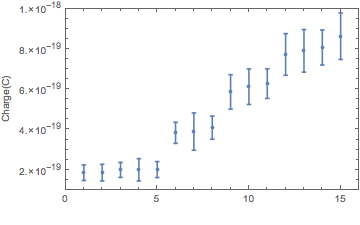
\includegraphics[width=8cm]{errorBarPlot.png}
\caption{Charge states of a selection of oil drops}
\label{fig:chargeplot}
\end{figure}


\begin{table}
\begin{tabular}{ |c|c| } 
 \hline
 Charge (C) & $\sigma$ \\ \hline\hline
$1.85292\times10^{-19}$ & $3.8477\times10^{-20}$ \\
$1.85615\times10^{-19}$ & $4.09597\times10^{-20}$ \\
$1.99147\times10^{-19}$ & $3.72199\times10^{-20}$ \\
$1.99801\times10^{-19}$ & $5.52185\times10^{-20}$ \\
$2.00892\times10^{-19}$ & $3.95016\times10^{-20}$ \\
$3.82999\times10^{-19}$ & $5.21442\times10^{-20}$ \\
$3.89048\times10^{-19}$ & $9.23826\times10^{-20}$ \\
$4.08603\times10^{-19}$ & $5.71004\times10^{-20}$ \\
$5.86004\times10^{-19}$ & $8.55453\times10^{-20}$ \\
$6.12047\times10^{-19}$ & $8.82026\times10^{-20}$ \\
$6.27298\times10^{-19}$ & $7.3251\times10^{-20}$ \\
$7.72017\times10^{-19}$ & $1.03229\times10^{-19}$ \\
$7.89952\times10^{-19}$ & $1.05625\times10^{-19}$ \\
$8.06608\times10^{-19}$ & $8.6788\times10^{-20}$ \\
$8.62615\times10^{-19}$ & $1.1525\times10^{-19}$ \\ \hline
\end{tabular}
\caption{Charge values and uncertainties}
\label{fig:chargetable}
\end{table}

By taking the mean of the values corresponding to each charge state and looking at the difference in these values, we observe that the magnitudes of the steps are integer multiples of a constant value. We calculate this value to be 
\[
    e = \SI{1.994e-19}{C}.
\]
There are several errors associated with this measurement, which will be
discussed in the next section.

\section{Error}
We now determine a systematic error on our measurement of $e$. From
equation~\eqref{eq:charge}, we see that the charge on each droplet is a function of the variables $E$, $v_f$, $v_r$, $p$, $a$, and $\eta$. By calculating the variances of each of these variables from the error propogation law, we may obtain a value for the standard deviation of the charge on each droplet. The errors associated with each charge calculation are listed in table~\ref{fig:chargetable}. Then, noting that our value of $e$ is a function of each of these individual charges, we apply the error propagation law again to obtain a final value of the uncertainty of our result. A table of the assumed and calculated uncertainties associated with each variable is shown in table~\ref{fig:errors}.
\begin{table}
\begin{tabular}{ |c|c| } 
 \hline
 Variable & $\sigma$ \\ \hline\hline
$V$ & $\SI{5}{V}$ \\
$T$ & $\SI{0.5}{K}$ \\
$p$ & $\SI{133.3}{Pa}$ \\
$\eta$ & $\SI{6.074e-16}{N.s/m^2}$ \\
$t$ & $\SI{0.05}{s}$ \\
$d$ & $\SI{0.05}{mm}$ \\ \hline
\end{tabular}
\caption{Variables and uncertainties}
\label{fig:errors}
\end{table}

The standard deviation of the measurement of $e$ is found numerically to be
\[
    \sigma_e = \SI{4.448e-20}{C}.
\]
The main source of error in our measurement comes from the uncertainties in the time and distance intervals used to calculate the velocities of the droplets. The low frame rate of screen recording contributes significantly to the error in the time interval, and the frame rate of the camera used to view the drops gave rise to uncertainties in the distance traveled by each drop. We estimate these uncertainties in the time and distance intervals to be $\sigma_t = \SI{0.05}{s}$ and $\sigma_d = \SI{0.05}{mm}$, respectively. We also accommodated for uncertainties in our measurements of the temperature, pressure, and voltage, although these errors had relatively small effects on our total systematic uncertainty.
\section{Conclusion}

We were able to calculate the value of $e$ to be
\[
    e = (1.994 \pm 0.445) \times 10^{-19} \,\si{C}.
\]
Comparing this with the known value of the electric charge $e$, $e_0 = \SI{1.602e-19}{C}$, we see that $e_0$ falls within one standard deviation of our measurement.
Thus, our experimentally determined value of $e$ agrees reasonably with the
known value.

\end{document}
